\documentclass{article}
\usepackage[utf8]{inputenc}
\usepackage{graphicx}
\usepackage[
backend=biber,
style=authoryear,
citestyle=authoryear
]{biblatex}
\renewcommand*{\bibfont}{\small}
\usepackage[normalem]{ulem}
\usepackage{fancyhdr}
\usepackage{multicol}
\usepackage[hidelinks]{hyperref}
 
\pagestyle{fancy}
\fancyhf{}
\rhead{Hypodermic needle after all?}
\lhead{Nicolai Berk}
\cfoot{\thepage}

\useunder{\uline}{\ul}{}

\addbibresource{PhD-Proposal.bib}


\usepackage{xcolor}

\title{Hypodermic needle after all? Individual-level Moderators of Media Framing Effects}
\author{Nicolai Berk\footnote{Doctoral Candidate, Dynamics Doctoral Program, Humboldt-Universität zu Berlin, \href{mailto:nicolai.berk@hu-berlin.de}{nicolai.berk@hu-berlin.de}}}
\date{May 2021}

\begin{document}

\maketitle


\begin{abstract}
    Scholars of political behaviour continue to debate the importance of the news media for citizens' opinion formation process. It has been argued that in today's media environment, persuasive effects of media coverage are unlikely, as viewers self-select into outlets whose coverage is in line with their preferences. At the same time, a growing body of evidence shows that endorsements and changing media content sometimes affect citizens' preferences, but not always. Current scholarship explains this with environmental conditions, such as the ability of consumers to discount for a newspaper's bias, which favour or inhibit the effectiveness of media coverage. This paper contributes to this debate by assessing how consumers' individual-level characteristics condition news framing effects. It does so by leveraging a sudden shift in the migration framing of the major German tabloid, \textit{Bild}. This case allows to assess the causal effect of changing news frames on survey respondents' migration attitudes and - using state-of-the-art text analysis tools - issue definitions, as well as conditioning characteristics.
\end{abstract}



\section{Motivation}

% This needs to be tailored more closely to the interest of media framing - currently, there is a lot more in here

How does the news media affect citizens' issue attitudes? Research on political behaviour has discussed this question for nearly a century. Classic theories of agenda setting hold that the attention devoted to issues in the news media will guide citizens to consider these issues important (\cite{McCombs1972}). Similarly, the literature on framing expects that the presentation of issues in the news media will affect recipients' opinions about these issues (\cite{Nelson1997}). Both theories suggest that media coverage strongly affects citizens' understanding of and opinions about politics.

A vast amount of evidence supports this notion of the importance of newspaper coverage for political behaviour. Observational evidence shows that newspaper exposure (\cite{Foos2020, Spirig2020}), endorsements of specific candidates (\cite{Ladd2009a, Chiang2011a}), coverage of specific topics (\cite{King2017}), reports on political parties (\cite{Boomgaarden2009, Devine2020}), internet access (\cite{Schaub2020}), and changes in television news content (\cite{Durante2012}) have affected which issues citizens care about, their opinion about these issues, and their voting behaviour. An even larger body of experimental work reports strong effects of issue framing on participants' issue attitudes (see \cite{Busby2019} for a recent overview).

Yet, a popular critique of these theories maintains that strong news effects are unlikely in the modern media environment, where consumers self-select into news sources of their liking. As a result, "most media users will rarely find themselves in the path of attitude-discrepant information". Even if consumers had to face such discrepant information, this should reinforce their existing views rather than persuade as they are used to a partisan media diet (\cite[724f]{Bennett2008}). Similarly, agenda setting effects are unlikely as a result of selective exposure (\cite{Lau2021}).

This "minimal effects" view is supported by a body of evidence as well. \citeauthor{Gentzkow2011} show that even historically, the entry and exit of newspapers in the US does affect turnout, but that the newspapers' slant does not affect either party's vote share. They conclude that "the persuasive effect of partisan newspapers is limited" (\citeyear[3011]{Gentzkow2011}). Recently, \citeauthor{Guess2021} incentivised participants of an online-panel to visit left- or right-leaning news websites, with no effect on opinions (\citeyear{Guess2021}). An experiment by \citeauthor{Lau2021} indicates that increasing the likelihood of encountering information about a fictitious candidate's stance on a given issue does not increase the importance of that issue in reaching a voting decision, directly contradicting theories of agenda setting. This lack of evidence echos a general critique of the external validity of framing experiments and other experimental evidence about opinion formation (\cite{Barabas2010, Busby2019, Leeper2020}).

This conflicting evidence begs the question: when can we expect media framing effects? \citeauthor{Chiang2011a} argue that endorsements from newspapers with ideological leanings neutral or opposite to the endorsed party/candidate should have stronger effects on voting behaviour, as voters discount the general bias of a newspaper (\citeyear{Chiang2011a}). \citeauthor{Spirig2020} shows that the takeover of a Swiss regional newspaper through a leading politician of the far-right and the subsequent change in its political slant had no effect on citizens' voting behaviour and suggests that this is a result of voters discounting the new owner's political slant and stopping to read the newspaper.

Prior experimental research also suggests that individual characteristics condition opinion stability (\cite{Converse1962, Zaller1992}). As a result, news framing should affect individuals differently. The goal of the present study is to assess whether changing news frames affect individual issue definitions and attitudes in a case where voters are unlikely to discount, and whether the strength of this effect is dependent on individual characteristics. This manuscript proceeds in three steps: the next section explains how I will operationalise framing, before I discuss possible individual-level moderators and formulate hypotheses.The last section describes the case of interest and briefly outlines my empirical strategy.


\section{Emphasis framing and the value-expectancy model of opinion formation}

While news slant is a very general concept, and sometimes operationalised as closeness to specific parties (\cite{Gentzkow2010}) or issue positions/tonality (\cite{Spirig2020}), framing theory provides a specific expectation about which treatment should affect which issue attitudes how. "Framing is the process by which a communication source, such as a news organisation, defines and constructs a political issue or public controversy" (\cite[567]{Nelson1997}). A "frame" is then the operating unit of this process, defining the issue at hand in a specific way. Different forms of frames have been conceptualised. When I talk about 'frames', I refer to \textit{emphasis frames}. These frames emphasise certain topics in relation to an issue, guiding the recipient to think about the issue with those considerations in mind that are promoted by the frame (\cite[153f]{Leeper2020}). For example, issues of increasing welfare contributions might be discussed with reference to inequality and providing chances to the poor, or by mentioning that higher welfare benefits might result in higher taxes. Individuals' support of a statement will differ dependent on the frame presented (\cite{sniderman2004structure}).

While this broad definition gives a first idea of what framing is about, the concept of emphasis framing has been criticised for being too broad and imprecise to contribute anything meaningful to the field (\cite{Scheufele2012}). To address this shortcoming, I follow the framing literature building on the \textit{value-expectancy model} (\cite{Ajzen2000, Nelson1997}). This model suggests that an attitude on a given issue is a function of two things: considerations and their respective weights. The evaluation of the issue is subdivided into a number of considerations (to which political scientists might refer as "valence issues") that will be easier to evaluate. For example, to evaluate whether a lockdown is necessary to battle the spread of Covid-19 in one's country, a person might consider the detrimental short-term effect on businesses and individuals' mental health (negative considerations), as well as the cost of overburdened hospitals and additional deaths (positive considerations, at least with respect to the evaluation of a lockdown). Individuals weigh each of these considerations to form an overall opinion on the subject. 

Figure \ref{fig:cogStor} visualises this logic. A given issue is associated with an attitude or evaluation $y$. The issue is related to a number of different considerations, each of which carries an associated evaluation $x_i$, e.g. that the prevention of overcrowded hospitals is a good thing. Each of these considerations is more or less associated with the issue. Based on the strength of this association $w_i$, a given consideration's evaluation is more or less reflected in the issue evaluation $y$, which is equal to the weighted sum of considerations. Emphasis framing affects the issue attitude $y$ by changing the weights of different considerations\footnote{Note that this concept of framing is identical to second-level or attribute agenda setting (\cite{Lopezescobar2017, McCombs2000}; see \cite[174]{Mclaren2018} for a discussion of the overlap of these literatures). I will stick to the framing perspective here as the literature is focused on issues rather than candidates' attributes, and the conceptualisation as frame allows to form expectations about citizens' reactions to changing news frames.}.

This operationalisation allows us to generate specific expectations about how frames in the news media affect respondents' issue opinions. When presented with an emphasis frame on a given issue, the respondents' cognitive association of the issue with the emphasised consideration should increase, thus changing the evaluation of the issue by increasing the importance of the consideration. If the consideration is positive (towards the issue), the attitude towards the issue should improve, and the opposite when it is negative. This also means that the definition of the issue (the cognitive image evoked when thinking of the issue) is changed by strengthening the association with the consideration.

% JB: I’m wondering if negative reference might help you with the definition. In our last colloquium you still got the criticism that framing was not well defined enough. I think you might be able to avoid a lot of the criticism (what makes framing different from issue ownership etc.) by addressing the contrast from framing from some of the more used concepts such as issue attention. Just an idea

% \footnote{I will stop here to outline the other chapters. However, a future version of this draft will discuss the cognitive basis of this model (considerations: affective storage as discussed by Taber and Lodge, Kunda; weights: physical cognitive association through Hebbian learning) and  whether this is a rational model (\cite{Ajzen2000, Druckman2001}).}.

\begin{center}
\begin{figure}
    \centering
    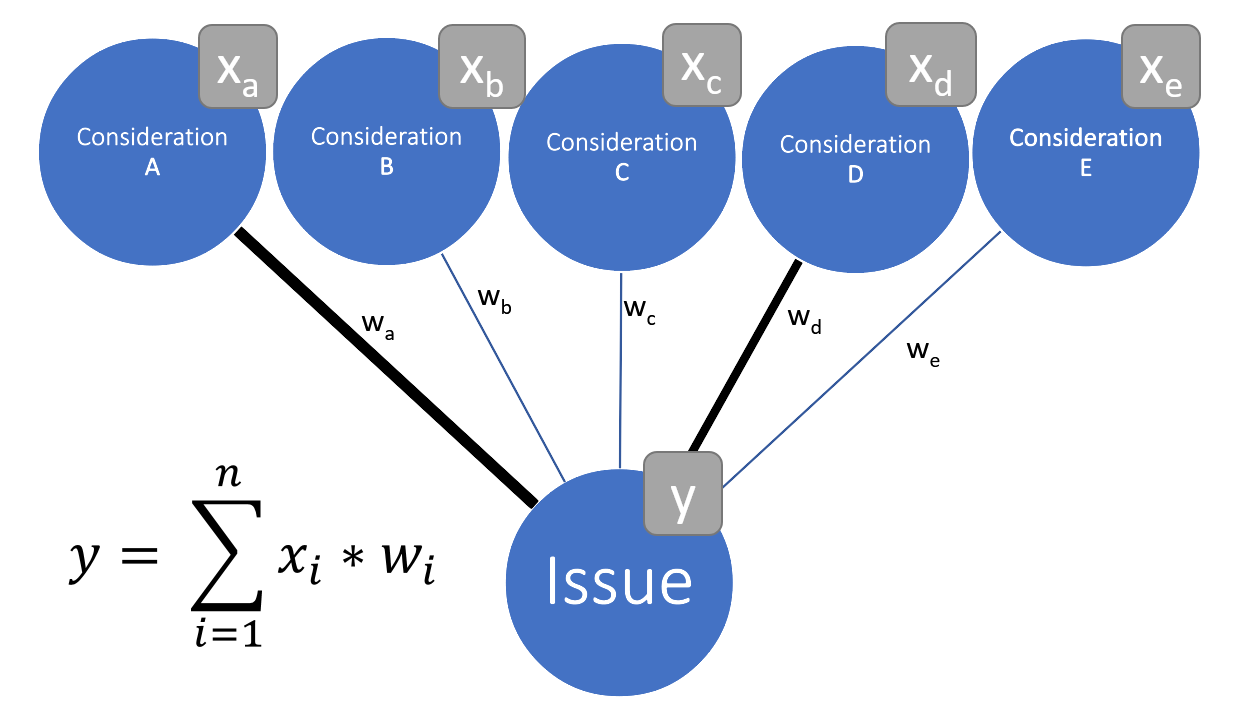
\includegraphics[width=\textwidth]{pres/vis/CognitiveStorage.png}
    \caption{The cognitive evaluation of an issue $y$ is determined by the strength of association $w_i$ with other concepts with existing evaluations $x_i$.}
    \label{fig:cogStor}
\end{figure}
\end{center}



\section{Susceptibility to framing effects}

As discussed before, my interest revolves not only around whether media frames affect respondents' issue definitions and attitudes, but also whether this effect is dependent on individual characteristics. As previous research indicates, individuals' attitude stability is dependent on their political knowledge (\cite{Converse1962}). If citizens have higher knowledge about political issues, they should rely less on the immediately available considerations presented in the news and more on memorised information about an issue instead (\cite{Zaller1992}). Hence, they should show a weaker inclination to respond to changing issue associations in the media. Similarly, the strength of pre-existing opinions about an issue has been shown to condition framing effects (\cite{Bechtel2015, Chong2013}). This means that only respondents with no clear opinion on an issue will show susceptibility to framing. 
% This might be attributed to higher knowledge about an issue or cue-taking from political parties. If the former is the case, the effect of pre-existing opinions should diminish when controlling for political knowledge, if the latter, controlling for partisanship should explain the relationship.

If the media environment conditions framing effects across time (\cite{Bennett2008}), it might also well be that individuals with different news consumption habits are differently affected by framing. While consumers with only a single source of news might - similar to citizens in the golden age of broadcast television - be more inclined to follow their news source's framing, those with a more balanced media diet from different sources might resist the changing framing.

% add motivated reasoners taking partisan cues

The next section lists the main hypotheses. Hypotheses 1 and 2 are based on the value-expectancy model of framing: if a reader is exposed to a given consideration through an emphasis frame, this consideration will feature more prominently in their definition of the issue. As a result of this, the consideration will also affect their issue attitude. 3 and 4a build on the viewer's choice framework. An extreme version of this framework could predict that, in response to the changing media framing, opinionated readers will seek out other news sources in line with their attitudes (see also \cite{Spirig2020}). If readers are solely dependent on the source of the frame (consuming no other newspaper), they will be more susceptible to framing. The two other conditioning variables - political knowledge and clear opinion - relate to the availability of frames in memory (4b \& 4c). Without a clear information about the issue or a position to identify with, receivers should be more likely to follow the frame. % add that motivated reasoning suggests that partisans are cue-takers ad will ignore frames

\section{Hypotheses}

\begin{enumerate}
    \item{When news coverage of an issue becomes more associated with specific considerations, these considerations will be more common in media consumers' definition of the issue.}
    \item{When news coverage of an issue becomes more associated with positive (negative) considerations, consumers will develop a more positive (negative) opinion towards the issue.}
    \item{When news coverage of an issue becomes more associated with positive (negative) considerations, those readers with conflicting attitudes towards the issue will stop reading the paper.}
    \item{The framing effect on attitudes (2) is only observable among respondents who...}
    \begin{enumerate}
        \item{\textit{have a limited media diet}.}
        \item{\textit{have low political knowledge}.}
        \item{\textit{had no clear opinion about the issue before}.}
    \end{enumerate}
    % \item{The moderating effect of pre-existing opinions can be explained by...}
    % \begin{enumerate}
    %     \item{\textit{political knowledge}}
    %     \item{\textit{partisanship}}
    % \end{enumerate}
\end{enumerate}


\section{Case and empirical strategy}

% \textbf{[HK: DROP EXOGENOUS LANGUAGE, DISTINGUISH FROM FOOS \& BISCHOF, THINK ABOUT DV REG CONTRIBUTION, SPILLOVER FROM BILD TO OTHER OUTLETS?]}

During the summer of 2015, the German tabloid \textit{Bild} dramatically changed it's framing of migration and refugees, calling for support for the newly arriving immigrants and attacking those promoting hate against refugees online (\cite{Bild2015Pranger, TagesspiegelBildPranger}), before starting the campaign 'We help - \#refugeeswelcome' (\cite{BildRefugeesWelcome}). With this move, the paper heavily diverged from its right-wing tradition. The major change in tone was largely ascribed to editor-in-chief Kai Diekmann, who had also invited a refugee family to live in his house (\cite{BR2015Diekmann}). In late 2015, Diekmann left for another position in the company, and was replaced by Tanit Koch, who promoted a more anti-immigrant tone of the paper. She was replaced two years later by \textit{Bild online}-editor Julian Reichelt (\cite{Spiegel2018Koch}), who amplified the tone further, which resulted in major criticism of the paper (\cite{Niggemeyer2018Bild, DLF2018Reichelt}).

I hope to exploit these communicative shifts in the paper's migration framing to assess the effects of media framing on readers' issue definitions, attitudes, and voting behaviour. If the migration framing changed in \textit{Bild} while other outlets maintained their framing, this presents an ideal case to estimate the causal effect of changes in media framing.

%  (the migration issue came up unexpectedly, Diekmann was promoted\footnote{\url{https://www.sueddeutsche.de/medien/boulevard-zeitung-tanit-koch-wird-chefredakteurin-der-bild-1.2723462}} and Tanit Koch apparently lost an internal power struggle with Julian Reichelt\footnote{\url{https://www.faz.net/aktuell/feuilleton/medien/chefredakteurin-tanit-koch-verlaesst-die-bild-15429101.html}})

I will rely on two major datasets to estimate the effect of this shift in migration framing:
\begin{itemize}
    \item \textit{Bild online} articles for the respective period (2013-2018) to measure the changes in migration framing.
    \item \textit{Bild} articles (print) would possibly provide a comparison and credibility check to compare the framing under Reichelt and Koch, as he was in charge of the online news, while she was in charge of the print paper\footnote{Not sure if this is entirely necessary, I haven't figured out where to get these yet - I thought maybe Lexis Nexis or the Bild Zeitung has an archive, I am grateful for suggestions though. The survey is asking for print and online news consumed, but i haven't looked into the data yet.}.
    \item Variables from the long-term online tracking survey of the German Longitudinal Election Study:
    \begin{itemize}
        \item \textbf{Respondents' media consumption.} This conditioning variable allows me to compare \textit{Bild}-readers to consumers of other media and to assess whether they were responsive to the paper's communicative shifts.
        \item \textbf{Open-ended 'most-important-problem' question (MIP).} This enables me to test whether respondents' associations with the migration issue changed.
        \item \textbf{Migration attitudes.} This variable indicates whether changes in migration framing in the media affect readers' assessment of political issues - the core claim of both the media effects and the framing literature.
        % \item \textbf{Vote decision.} This dependent allows to test whether changes in media frames affected voting behaviour.
        \item \textbf{Political Knowledge.} This independent variable allows to test whether susceptibility to framing is dependent on political knowledge.
        \item \textbf{Media diet.} This independent variable indicates whether the respondent consumes additional news sources. Allows to test whether susceptibility to framing is dependent on having alternate news sources.
    \end{itemize}
\end{itemize}

While I collected the \textit{Bild} articles myself using webscraping, the survey data is provided by the German Longitudinal Election Study (GLES). The long-term online tracking consists of quarterly surveys of a random sample of about 1,000 respondents beginning in 2009 and ending in 2017 (\cite{GLES2019LongTermTracking}). Importantly, it contains questions on media usage, specifically if respondents read \textit{Bild}, as well as open-ended questions about the most important problem, attitudes towards migration (later on also specific batteries on attitudes towards refugees), and political knowledge in most waves.

This provides great data to estimate whether the issue definitions and attitudes of \textit{Bild} readers changed in response to changing coverage in 2015 and 2016, but the data has limitations. Most importantly, the survey does not interview the same respondents again. This means that I won't be able to assess hypotheses 3 and 4c. To test these hypotheses, the GLES Panel survey might be used. This data only covers 2016-2020, which includes the last but likely weakest treatment (Reichelt replaced Koch; see figure \ref{fig:gles}). Additionally, the number of respondents in the longterm online tracking is rather small given that my group of interest is \textit{Bild} readers and the hypothesised interaction effects. These should constitute 150-200 respondents per wave. Again, the panel would provide a solution, with 2,000-4,000 \textit{Bild} readers per wave (15-20\% of respondents).

\begin{figure}
    \centering
    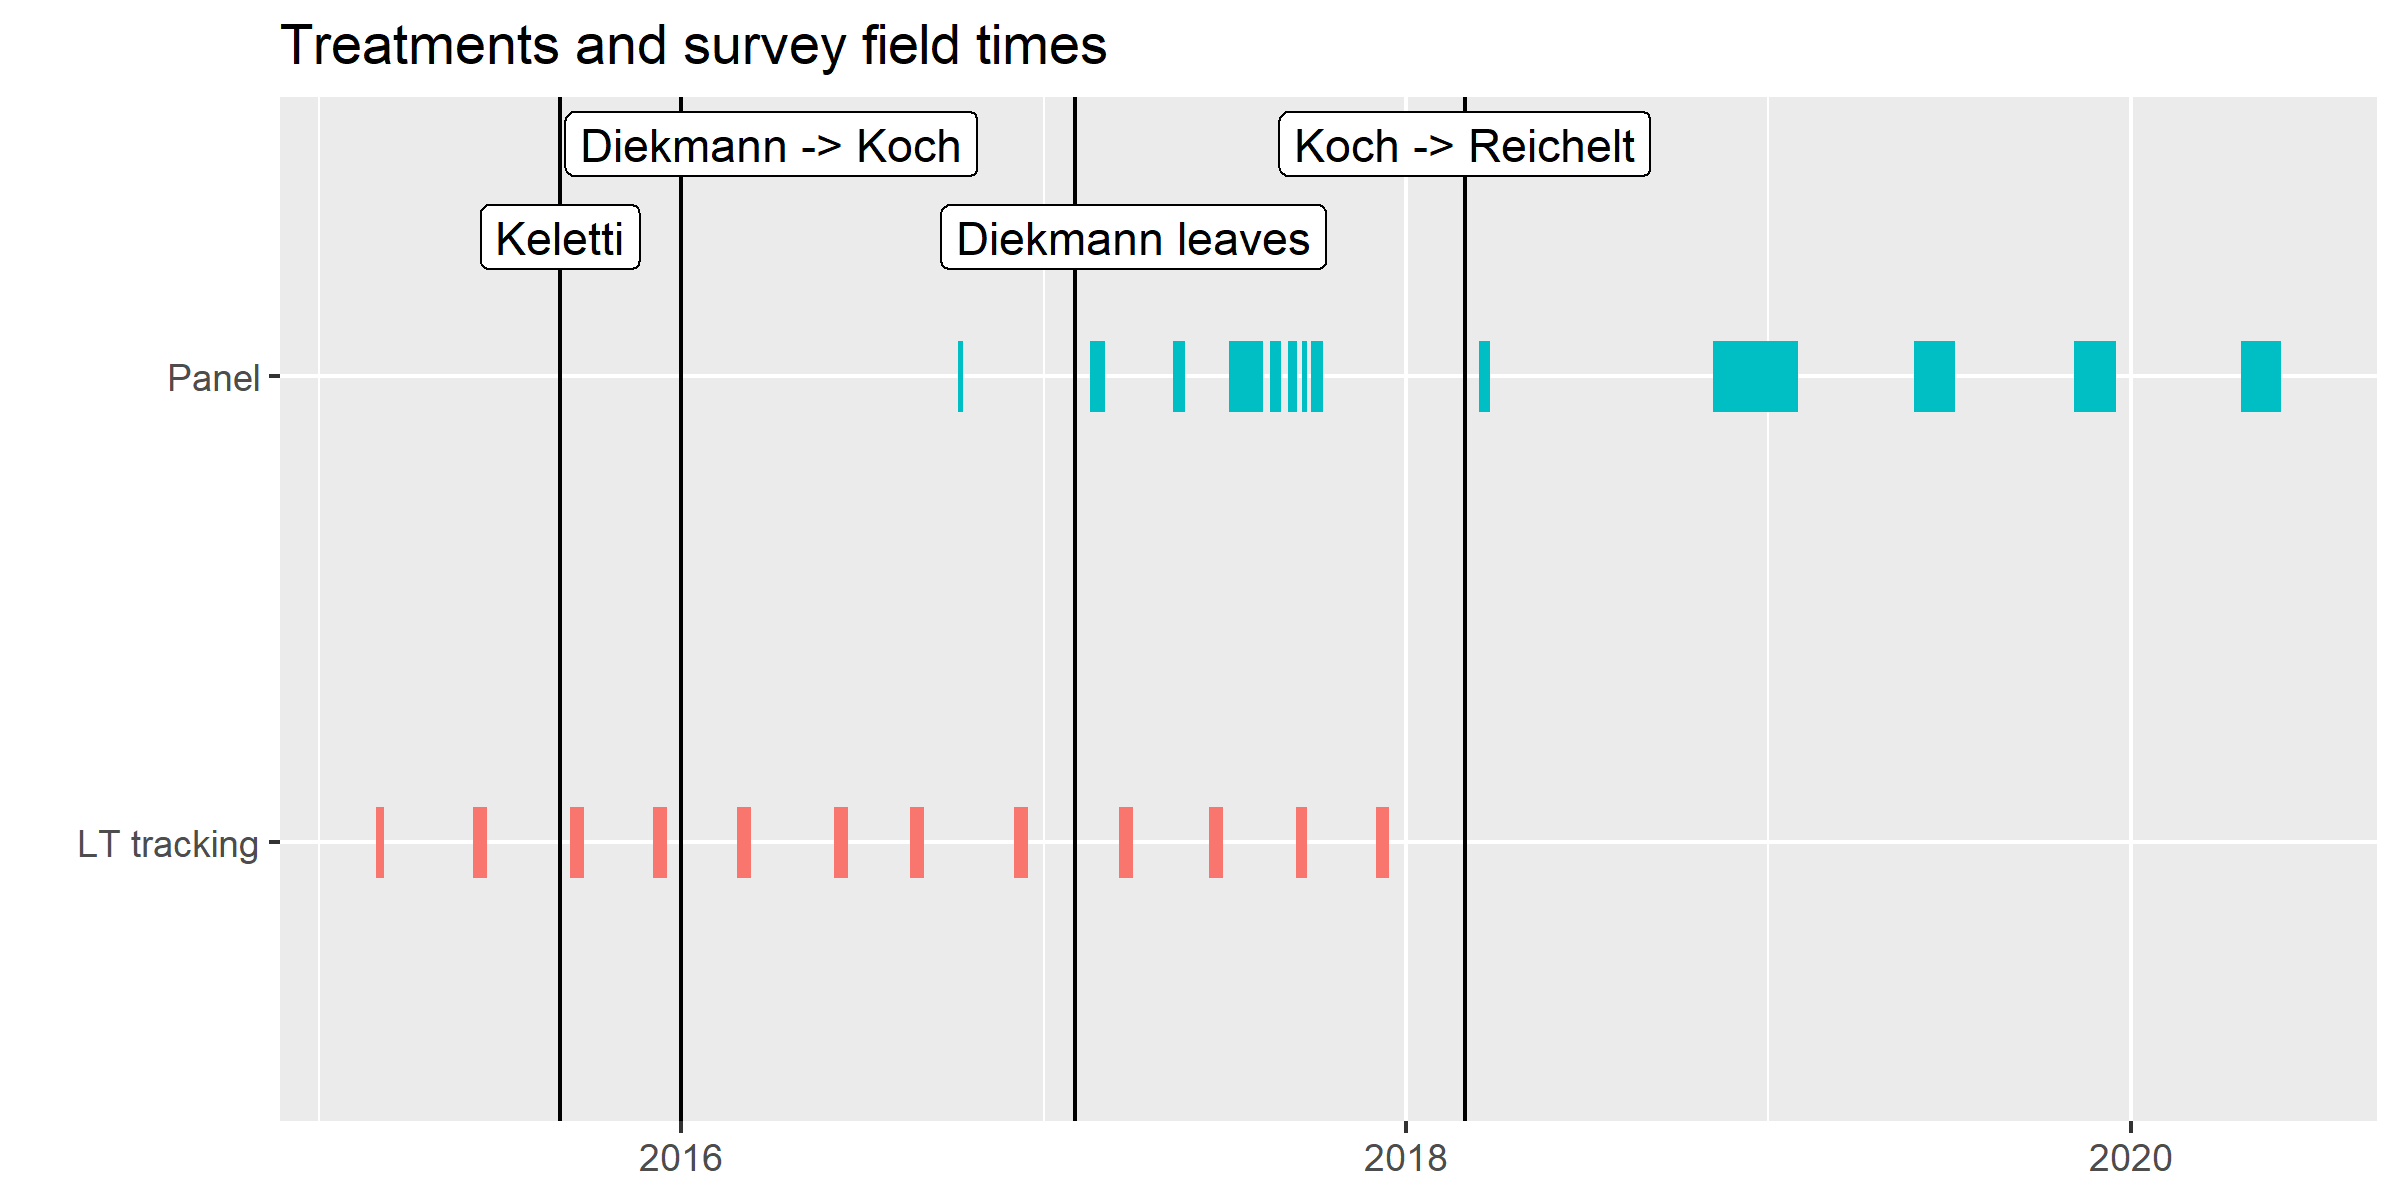
\includegraphics[width=\textwidth]{pres/vis/gles_treatments.png}
    \caption{Relative timing of possible shifts in migration framing and survey field times.}
    \label{fig:gles}
\end{figure}

Which treatment is viable will have to be decided based on an empirical comparison of the migration frames in \textit{Bild} to those in other newspapers. If the framing in \textit{Bild} diverges from a parallel trend with the framing of other newspapers, the treatment is viable. I have not yet decided on how to measure framing here. The most straightforward approach would in my opinion be to pre-select migration content (in all newspapers) with a supervised machine-learning classifier. Then either identify pre-defined frames (e.g. humanitarian frame, crime, ...) using a dictionary approach, possibly with dictionary extension using word embeddings; or use factor analysis/structural topic modelling to identify frames inductively (\cite{Nicholls2020}). Either way, I would have to select relevant positive and negative frames to track across time, either a priori or as a selection from the topic model. If e.g. the change from Diekmann to Koch corresponded with a major shift in framing (e.g. lower emphasis of the humanitarian frame, more discussion of crime in relation to immigration/integration), relative to other newspapers, this would indicate a viable treatment.

After the selection of the viable treatment, a differences-in-differences design (DiD) will be estimated:

$$ y = \beta_1 * T + \beta_2 * B + \beta_3 * T * B $$

Where $y$ is the dependent (migration association or attitude), $T$ indicates whether the interview took place after the treatment/shift in migration framing, and $B$ indicates whether the respondent is a \textit{Bild}-reader. This means that the average of the dependent variable among \textit{Bild}-readers following the treatment is compared to non-\textit{Bild}-readers, both before and after the treatment, and \textit{Bild}-readers before treatment. $\beta_3$ - the quantity of interest - is then equal to the difference-in-differences, meaning the change in the dependent variable from before to after treatment, adjusted for the change among the control group (non-\textit{Bild} readers).

While the implementation is relatively straightforward for the migration attitude-variable using a five-point Likert scale, it is more complicated for the association of concepts with migration. Whether this can be measured is highly dependent on the number of responses discussing migration in the open answers to the most-important problem question. If possible, several surveys preceding and following the treatment should be pooled to increase the number of respondents. 

To estimate the changing meaning of concepts in text, word embeddings have emerged as a state-of-the-art method. This method allows the numerical representation of semantic meaning in a high-dimensional vector-space. Those words with more similar meanings will occur closer together in the vector space, which allows the identification of changing meaning across corpora. However, these models require extensive training data (\cite{Rodman2019}). Recent work has tackled this problem by mapping embeddings into pre-trained, high-quality embedding spaces (\cite{Khodak2018}). This opens the possibility to quantitatively assess changing meaning in applications with few observations, such as open survey responses. Building on this work, \citeauthor{Rodriguez2020} have developed \textit{embedding regression}, which allows to express changing meanings as a function of covariates (\citeyear{Rodriguez2020}). Using the DiD to estimate these changes in meaning, it will be possible to understand how \textit{Bild}-readers' understanding of migration changed following the treatment, compared to changes in the control group.

This will be compared to the outputs of the embedding regression for DiD with newspaper data, comparing migration framing in the \textit{Bild} before and after treatment to other newspapers before and after treatment. If the changes in the definition of migration indicated by the DiD are similar in the newspaper data and the survey responses, this constitutes strong evidence for a direct transmission of news frames into the issue definitions of consumers of these news.

Lastly, another model with political knowledge and the diversity of the media diet as moderators and migration attitude as the dependent will be estimated to test hypotheses 4a and 4b.

% \textbf{[AV:  You should add info on who the part of people who actually write a lot are. Are they representative of BILD readers? Reichelt: Move from online editor to main editor? Does she have no influence on frames already? Do you have data on how ppl consume media?]}

\newpage

\printbibliography

\end{document}
